\documentclass[12pt]{article}
%%%%%%begin preamble
\usepackage[hmargin=1in, vmargin=1in]{geometry} % Margins
\usepackage{hyperref}
\usepackage{url}
\usepackage[numbers]{natbib}
\usepackage{graphicx}
\usepackage{amsmath}
\usepackage{amsfonts}
\usepackage{amssymb}
\usepackage{wrapfig}

\usepackage{multicol}
\usepackage{etoolbox}
%\patchcmd{\thebibliography}{\section*{\refname}}
%    {\begin{multicols}{2}[\section*{\refname}]}{}{}
%\patchcmd{\endthebibliography}{\endlist}{\endlist\end{multicols}}{}{}


\usepackage[normalem]{ulem}
\usepackage{xcolor}
\newcommand{\edit}[2]{\textcolor{purple}{\sout{#1} \textbf{#2}}}

\hypersetup{
  colorlinks   = true,
  %citecolor    = blue
  citecolor    = blue
  % gray is not being found!?!
  % gray is found if pdfpages is used... crap.
  %citecolor    = grey
  %citecolor    = Gray
}


%% headers
\usepackage{fancyhdr}
\pagestyle{fancy}
\fancyhf{} % sets both header and footer to nothing
\lhead{Evan H. Anders}
\rhead{Research Statement}
\cfoot{\footnotesize{\thepage}}
%\pagestyle{empty}
%\pagenumbering{gobble}
%\renewcommand*{\thefootnote}{\fnsymbol{footnote}}

\renewcommand{\vec}{\ensuremath{\boldsymbol}}
\newcommand{\dedalus}{\href{http://dedalus-project.org}{Dedalus}}
\newcommand{\del}{\ensuremath{\vec{\nabla}}}
\newcommand{\scrS}{\ensuremath{\mathcal{S}}}

\newcommand{\prf}{PRF}
\newcommand{\prr}{PRR}
\newcommand{\ssr}{SSR}
\newcommand{\araa}{ARAA}
\newcommand{\mnras}{MNRAS}
\newcommand{\aap}{A\&A}
\newcommand{\apjl}{ApJL}
\newcommand{\apj}{ApJ}
\newcommand{\apjs}{ApJL}

\newcommand{\sct}[1]{\vspace{0.3cm}\hspace{-\parindent}\textbf{\underline{#1}}\hspace{0.3cm}}

%\newcommand{\nosection}[1]{%
%  \refstepcounter{section}%
%  \addcontentsline{toc}{section}{\protect\numberline{\thesection}#1}%
%  \markright{#1}}
%\newcommand{\nosubsection}[1]{%
%  \refstepcounter{subsection}%
%  \addcontentsline{toc}{subsection}{\protect\numberline{\thesubsection}#1}%
%  \markright{#1}}

%\usepackage{atbegshi}
%%%%%%end preamble


%Make bibliography 2col
\bibliographystyle{apj_small}
\makeatletter
\renewenvironment{thebibliography}[1]
     {\begin{multicols}{2}[\paragraph*{\refname}\vspace{-0.1in}]%
      \@mkboth{\MakeUppercase\refname}{\MakeUppercase\refname}%
      \list{\@biblabel{\@arabic\c@enumiv}}%
           {\settowidth\labelwidth{\@biblabel{#1}}%
            \leftmargin\labelwidth
            \advance\leftmargin\labelsep
            \@openbib@code
            \usecounter{enumiv}%
            \let\p@enumiv\@empty
            \renewcommand\theenumiv{\@arabic\c@enumiv}}%
      \setlength{\itemsep}{-2pt}
      \sloppy
      \clubpenalty4000
      \@clubpenalty \clubpenalty
      \widowpenalty4000%
      \sfcode`\.\@m}
     {\def\@noitemerr
       {\@latex@warning{Empty `thebibliography' environment}}%
      \endlist\end{multicols}}
\makeatother



\begin{document}
\thispagestyle{fancy}

\sct{Context \& Aims}
Current and next-generation space- and ground-based observatories are revolutionizing precision observations in astrophysics.
Discoveries ranging from exoplanets to black holes rely on high-precision stellar evolution models for calibration \citep{mesa6}, and convection introduces uncertainty into these models.
Mixing at the convective core boundary of massive stars ($M_* \gtrsim 1.1 M_\odot$) leads to core mass uncertainties of up to 70\% \citep{kaiser_etal_2020}, making the evolutionary pathway of a star from birth to death unclear.
Strange iron-opacity-driven convection in the outer layers of massive stars can also inflate the stellar surface thereby altering mass loss via winds \citep{kohler_etal_2015}.
These processes result from nonlinear 3D convection, which is poorly modeled in stellar evolution calculations and theoretical prescriptions.


\textbf{The goal of my research plan is to build a next-generation set of global and local 3D numerical simulations, which will answer the following questions:}\vspace{-0.2cm}
\begin{enumerate}
    \item How large are convective cores in massive stars? \vspace{-0.2cm}
    \item How does iron-bump convection affect the stratification and surface temperature of massive stars?
        And, does iron-bump convection block gravity wave signals?
\end{enumerate}

\sct{My Prior Research}
\textbf{My research is rooted in fluid dynamics and inspired by observations of stars.}
I use the \emph{Dedalus} \citep{burns_etal_2020} pseudospectral code to create well-posed numerical experiments which I use to learn about mixing processes like convection in stars.
\textbf{When I was a graduate student, I focused on fundamental studies of convection.}
I studied heat transport in compressible convection with  \citep{anders_etal_2019_rot} and without \citep{anders_brown_2017} rotation.
I studied how fast convection interacts with the slow evolution of the background thermal structure in convective regions \citep{anders_etal_2018,anders_etal_2020}.
I also studied convection at the smallest scales, examining individual downflows in the Sun's convection zone \cite{anders_etal_2019_thermals}.
\textbf{As a postdoctoral fellow at Northwestern, I have connected my theoretical research with modern observational puzzles.}
I have formed collaborations with observers and 1D modelers alike to understand what sets the position of a convective boundary \citep{anders_etal_2022b}, and I have discovered the process that inflates the convective cores of stars relative to standard models \citep{anders_etal_2022a}.
I am now finishing a project focusing on gravity wave generation by core convection and the observable signals of these waves, for direct comparison with e.g., asteroseismic observations.

\vspace{0.1cm}
\sct{Future Focus I: Convective Boundary Mixing}
Observations demonstrate a need for improved models of convective boundary mixing (CBM) \citep{johnston2021}.
For example, an unexplained mass-dependent CBM is required to reproduce observed eclipsing binary populations  \citep{claret_torres_2019}.
Asteroseismology also allows us to directly probe near-core CBM, revealing extensive mixing occurs near convective core boundaries \citep{michielsen_etal_2019, pedersen_etal_2021}.
The amount of CBM used in a stellar evolution model modifies the evolution of a star's luminosity and effective temperature as well as the mass of the eventual remnant that it leaves behind \citep{castro_etal_2014,higgins_vink_2019}.


To understand the fluid dynamical picture behind CBM, I will create simulations of the cores of massive stars using the \emph{Dedalus} \citep{burns_etal_2020} code.
These simulations will differ from past simulations of massive stars, because they will include the full ``ball'' geometry of the convective core, they will employ the fully compressible equations without any luminosity boosting, and they will be relaxed into thermal equilibrium (See Fig.~\ref{fig:star} for a preliminary example of one of these simulations).
\emph{Dedalus} was recently updated with the state-of-the-art ability to simulate flows that pass through the coordinate singularity at $r = 0$ in spherical coordinates \citep{vasil_etal_2019,lecoanet_etal_2019}; most prior codes used a spherical shell geometry with a small interior ``cutout'' of the core.
Our implicit-explicit (IMEX) timestepping scheme allows us to circumvent timestepping restrictions from fast sound waves \citep{anders_brown_2017}, so we can take fast timesteps without boosting the luminosity as many prior simulations have done.
Evolving a simulation to thermal equilibration using classic timestepping techniques can take thousands of convective overturn timescales \citep{anders_etal_2022a,anders_etal_2022b}.
Fortunately, I have developed methods of ``accelerated evolution'' \citep{anders_etal_2018}, which self-consistently equilibrate simulations using an order of magnitude fewer cpu-hours than traditional timestepping.



\begin{wrapfigure}{r}{0.5\textwidth}
  \begin{center}
      \vspace{-1.6cm}
    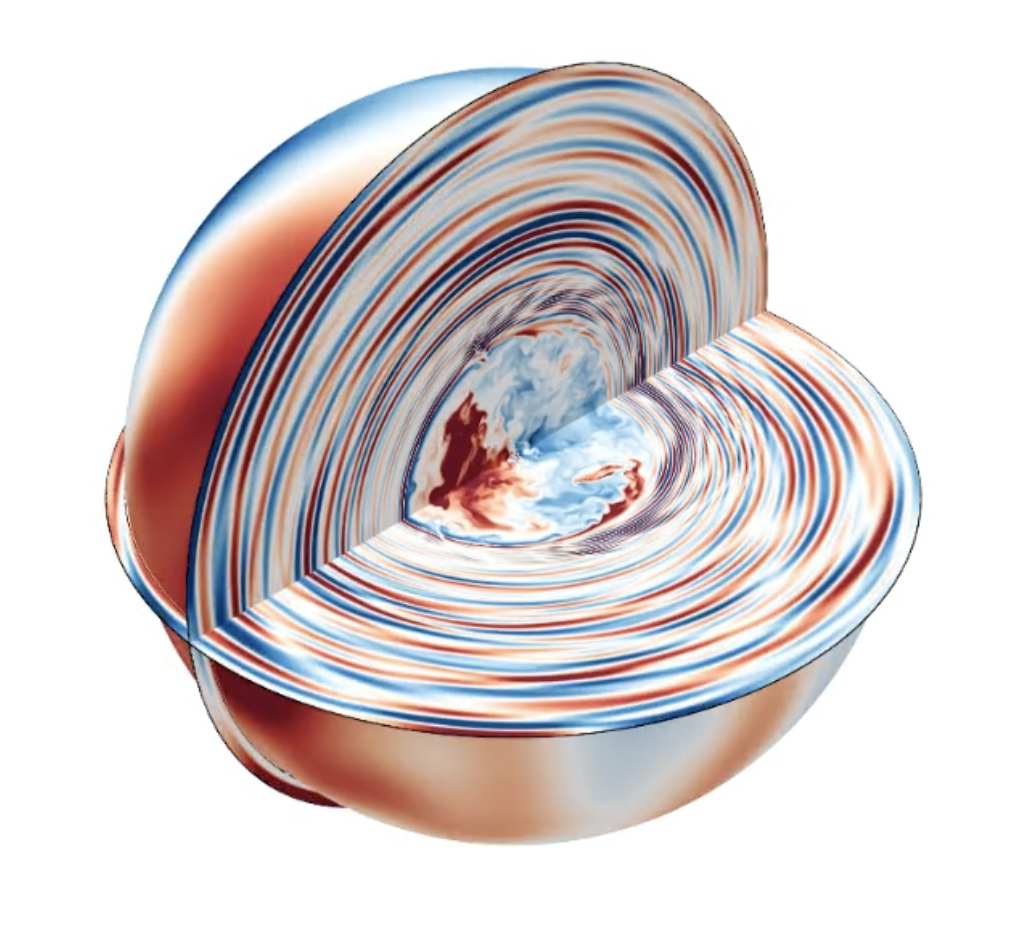
\includegraphics[width=0.45\textwidth]{dedalus_massive_star.png}
      \vspace{-1.3cm}
  \end{center}
    \caption{A simulation I ran in \emph{Dedalus} of a {$40 \,M_{\odot}$} star. 
    The entropy field is visualized; red is hot and buoyantly rises, blue is cold and falls. 
    We see a convective core with a strong dipole flow and an outer radiative envelope with internal gravity waves. \label{fig:star}}
    \vspace{-0.5cm}
\end{wrapfigure}
I will study CBM in fully compressible simulations whose background stratifications are based upon \emph{MESA} (Modules for Experiments in Stellar Astrophysics) models of massive stars.
I will study non-rotating and rotating stars with masses varying in the range $M_* = 1.1-40 M_{\odot}$ (the lowest masses where convective cores appear, up to high masses).
My results will calibrate a 1D implementation of convective boundary mixing, which I will then implement into the open-source \emph{MESA} software instrument.
Throughout this process, I will build my simulation code with ease-of-use for the user in mind, and this code will be made publicly available and citeable so that the community has access to a robust tool for studying fluid dynamics in massive stars.

\textbf{\underline{\emph{Deliverable:}} The first rotating, 3D simulations of core convection that include $\boldsymbol{r = 0}$ and reach thermal equilibrium.}

\sct{Future Focus II: Optically thick, low-efficiency Iron-Bump Convection.}
In addition to vigorous core convection, massive stars have opacity-driven convective shells in their envelopes \citep{cantiello_etal_2009}.
For stars with masses $\gtrsim 8 M_{\odot}$, an ``Iron-Bump Convection Zone'' (FeCZ) appears as a result of the opacity of iron.
These convection zones are odd: they approach the Eddington luminosity limit, are very thin, and exhibit high-Mach number, turbulent flows \citep{jermyn_etal_2022_atlas}.
%However, unlike the convection zones at the surface of lower-mass stars (e.g., the Sun), these convection zones generally appear at high optical depths \citep[fig 59 of][]{jermyn_etal_2022_atlas}.
This odd convection has not been studied in detail, but the presence of these convection zones influences the stellar structure and evolution appreciably \citep{kohler_etal_2015}.


Numerical simulations of these convection zones are extremely limited.
Those simulations which exist were performed using \emph{Athena} \citep{jiang_etal_2015, schultz_etal_2020} and demonstrate interesting dynamics and thermodynamics.
Unfortunately \emph{Athena}'s robust inclusion of full radiative hydrodynamics makes these simulations very expensive.
FeCZs are generally at high optical depth, and so simpler approximations for the radiative transfer can be used \citep{jermyn_etal_2022_atlas}.
I will incorporate iron-bump opacity effects into \emph{Dedalus} under various simplifying radiative transfer approximations.
I will work with \emph{Athena} experts at Princeton like Prof.~Jim Stone at the IAS to benchmark and validate my \emph{Dedalus} simulations against \emph{Athena} simulations to determine the range of stars where it is valid to approximate radiative transfer processes as optically thick.
After validating my code, I will study the high-Mach number convection in FeCZs in simulations spanning stellar masses from $8-60 M_{\odot}$ and at various stellar ages.
Flows in the FeCZ can support a large dynamic pressure, which can inflate the star; I will study how this turbulent pressure component varies across the HR diagram.
I will calibrate a prescription for how the turbulent pressure modifies the background pressure, incorporate this into \emph{MESA}, then study the observable consequences of this pressure.
I am particularly interested in how this pressure modifies the star's effective temperature, and the consequences that has for wind-driven mass loss.

Seperately, there is a current debate about whether the source of ``red noise'' on hot, massive stars \citep{bowman_etal_2019} is gravity waves generated in the convective core or turbulence generated by FeCZs \citep{cantiello_etal_2021}.
Existing FeCZ simulations generate turbulent fields which could explain red noise signals as well as ``macroturbulence'' signals \citep{schultz_etal_2022,schultz_etal_2022b}.
Simulations of core generated gravity waves \citep{edelmann_etal_2019,horst_etal_2020} have also shown promising comparisons with red noise, but do not include the FeCZ, and so do not capture how the FeCZ modifies gravity wave signals from the core.
I will study how gravity wave signals generated below the FeCZ change as they pass through this turbulent convection zone.
I will include the stable radiative zones surrounding the FeCZ in my simulations and force a spectrum of gravity waves below the FeCZ, then measure how these waves are modified by the turbulent convection in the FeCZ.

\textbf{\underline{\emph{Deliverable:}} The first 3D simulations of FeCZs across the HR diagram.}

\sct{Connections at Princeton}
Princeton is the ideal location for me to carry out this work.
I'm particularly excited to collaborate with Prof.~Eliot Quataert, who has expertise studying convective boundary mixing and convective wave generation and would be a key collaborator to help me unravel the questions I have discussed.
I also look forward to extensive collaboration with Prof.~Jim Stone, who I have spoken with briefly about the dynamics of FeCZs and who is keen on comparing \emph{Athena} and \emph{Dedalus} in these strange convection zones.
I hope to expand my research horizons and forge many collaborations with the broad network of scientists in Princeton.
For example, I'd be excited to explore applications of \emph{Dedalus} to planetary atmospheres with Prof.~Adam Burrows, and I'd be excited to forge interdisciplinary collaborations with geophysicists like Drs.~Jeevanjee and Donner at GFDL.

{\scriptsize
\bibliography{biblio}
}
\end{document}
